%Copyright �2019 Christopher M Jermaine (cmj4@rice.edu), and Risa B Myers  (rbm2@rice.edu)
%
%Licensed under the Apache License, Version 2.0 (the "License");
%you may not use this file except in compliance with the License.
%You may obtain a copy of the License at
%
%    https://www.apache.org/licenses/LICENSE-2.0
%
%Unless required by applicable law or agreed to in writing, software
%distributed under the License is distributed on an "AS IS" BASIS,
%WITHOUT WARRANTIES OR CONDITIONS OF ANY KIND, either express or implied.
%See the License for the specific language governing permissions and
%limitations under the License.

\documentclass[11pt]{article}
%\documentclass[12pt]{amsart}
%\usepackage{latex8}
\usepackage{fullpage}
\usepackage{times}
\usepackage{url}
\usepackage{epsfig} 
%\usepackage{latexsym}
\usepackage{subfigure}
\usepackage{graphicx}
\usepackage{titlesec}
\usepackage{multirow}

\titlespacing{\section}{0pt}{3mm}{1mm}
\titlespacing{\subsection}{0pt}{2mm}{0.5mm}
\titlespacing{\subsubsection}{0pt}{2mm}{0.8mm}

%\topmargin 0.75in 
%\oddsidemargin -0.04in
%\textwidth 6.5in
%\textheight 9.0in 
%\setlength{\textheight}{23.1cm}
%\setlength{\textwidth}{17.0cm}

\newcommand{\muhat}{\hat{\mu}}
\newcommand{\sigmahat}{\hat{\sigma}}
\newcommand{\todo}[1]{[\textbf{TODO: #1}]}
\newcommand{\eat}[1]{} % TO MAKE LARGE BLOCKS OF TEXT INVISIBLE
\newcommand{\sz}[1]{\lvert#1\rvert}
\newcommand{\card}[1]{\lvert#1\rvert}
\newcommand{\xp}[2]{P \if*#1\else^{#1}\fi \if*#2\else_{\! #2}\fi}
\newcommand{\pr}[3]{\xp{#1}{#2}\left\{\,#3\,\right\}}
\newcommand{\prl}[3]{\xp{#1}{#2}\{\,#3\,\}}
\renewcommand\:{\colon} % for use with \sset, etc.
\newcommand{\sset}[1]{\left\{\,#1\,\right\}}
\newcommand\xD{\mathcal{D}}
\newcommand\xP{\mathcal{P}}
\newcommand\xS{\mathcal{S}}
\newcommand\xbar{\bar x}
\newcommand\vbar{\bar v}
\newcommand\xmax{{x_{\text{max}}}}
\newcommand\eps{\epsilon}
\newcommand{\eeblk}{\hbox{\lower 1pt \vbox{\hrule width6pt\hbox to
  6pt{\vrule height5pt depth1pt \hfil\vrule height5pt depth1pt} \hrule
  width6pt} \unskip}}
\newcommand{\eblk}{{\unskip\nobreak\hfil\penalty50
  \hskip1em\hbox{}\nobreak\hfil\eeblk
  \parfillskip=0pt\finalhyphendemerits=0\par}}
\newtheorem{xample}{Example}
%\newenvironment{example}{\begin{xample}\em}{\eblk\end{xample}}
\makeatletter
\newenvironment{sql}%
 {\vskip 5pt\begin{list}{}{%
  \setlength{\topsep}{0pt}\setlength{\partopsep}{0pt}\setlength{\parskip}{0pt}%
  \setlength{\parsep}{0pt}\setlength{\labelwidth}{0pt}%
  \setlength{\rightmargin}{0pt}\setlength{\leftmargin}{0pt}%
  \setlength{\labelsep}{0pt}%
  \obeylines\@vobeyspaces\normalfont\ttfamily%
  \item[]}}
 {\end{list}\vskip5pt\noindent}
\makeatother
\newcommand{\bpar}[1]{\vskip 5pt\noindent\textbf{#1}\hskip 1em}
\newcommand\yN{{\tilde N}}
\newcommand\yX{{\tilde X}}
\newcommand\ymu{{\tilde\mu}}
\newcommand\ysigma{{\tilde\sigma}}


\newcommand{\goodgap}{
        \hspace{\subfigtopskip}
        \hspace{\subfigbottomskip}
}

%\renewcommand{\baselinestretch}{0.99}

\newtheorem{definition}{Definition}
\newtheorem{Rule}{Rule}
\newtheorem{lemma}{Lemma}
\newtheorem{theorem}{Theorem}
\newtheorem{problem}{Problem}
\newtheorem{example}{Example}
\newtheorem{optimization}{Optimization}
\newtheorem{observation}{Observation}
\newtheorem{corollary}{Corollary}

\newcommand{\qed}{\hspace*{\fill}
           \vbox{\hrule\hbox{\vrule\squarebox{.667em}\vrule}\hrule}\smallskip}

\long\def \ignoreme#1{}

\def\qed{\hfill \mbox{\rule[0pt]{1.5ex}{1.5ex}}}



\begin{document}
%\maketitle
%\pagestyle{empty}

\begin{center}
{\bf \huge{Spark AWS lab}}
\end{center}


\vspace{10 pt}

\section{Description}

This section is a high level overview. 

In this lab, you will:
\begin{enumerate}
\item Create an AWS EMR cluster
\item Upload a PySpark program onto the cluster
\item Run a Spark job
\item Check out the output on HDFS (Hadoop Distributed File System).
\end{enumerate}
	Note: this assumes you have previously signed up for an Amazon account. See Piazza!

\section{Create your Key Pair}
To connect to the cluster you will create later, you need a Key Pair as an identity.
\begin{enumerate}
\item Go to Amazon’s AWS website (aws.amazon.com).
\item Sign in with your user name and password. Go to EC2 (you can reach EC2 from the AWS services search text box).
\item Click ``key pairs''.
\item Click ``Create Key Pair''.
\item Pick a key pair name that is likely unique to you (such as the name of your eldest child, or your last name, so that it is unlikely that you will forget it). Type it in, and click ``Create''.
\item This should create a ``.pem'' file that you can download. You will subsequently use this .pem file to connect securely to a machine over the internet. 
\end{enumerate}

\section{Start Up a Cluster}

\begin{enumerate}
  \item Click the AWS at the upper left of the dashboard to get back to the
    main menu. Then, search for or click ``EMR''. This stands for ``Elastic Map
    Reduce.''
  \item Click ``Create cluster''.
  \item Choose the software configuration that includes Spark 2.4.0, as shown
    in Figure \ref{fig:aws-emr-spark}
  \item For the Master node, you want an m4.large machine. If you are
    interested, you can find a list of all instance types at
    https://aws.amazon.com/ec2/instance-types/.  Each m4.large machine has 4
    CPU cores and 8GB of RAM. For the Core workers, you want 2 m4.large
    machines.
  \item Under ``Security and access'', it is really important to choose the EC2
    key pair that you just created. \textbf{ This is important: if you do not
      do this, you won’t be able to access your cluster.}
  \item Click ``Create Cluster''. Now your machines are being provisioned in
    the cloud! You will be taken to a page that will display your cluster
    status. It will take a bit of time for your cluster to come online. You can
    check the status of your cluster by clicking the little circular update
    arrow at the top right.
   \item  Once your cluster is running, you need to make it so that you can connect via SSH. Under ``Security and Access'' (not a tab on the side, just a heading at the lower left), go to ``Security groups for Master'' and click on the link. In the new page, click on the row with Group Name = ``ElasticMapReduce-master''. At the bottom, click on the Inbound tab. Click on ``Edit''. Click ``Add Rule''. Then select ``SSH'' in the first box and ``Anywhere'' in the second. Click save.

\end{enumerate}

Note: the very first time that create a cluster, it may take 15 minutes or
more for the cluster to begin, and Amazon makes sure your account is valid.
Take the opportunity to update your Facebook or chat with your neighbor. As
soon as your master node changes to ``bootstrapping'', you are ready to go.

Note: if you ever want to get back to the page that lists all of your EMR
clusters, just click the ``AWS'' at the top left, then enter or click ``EMR''.

\begin{figure}
  \centering
  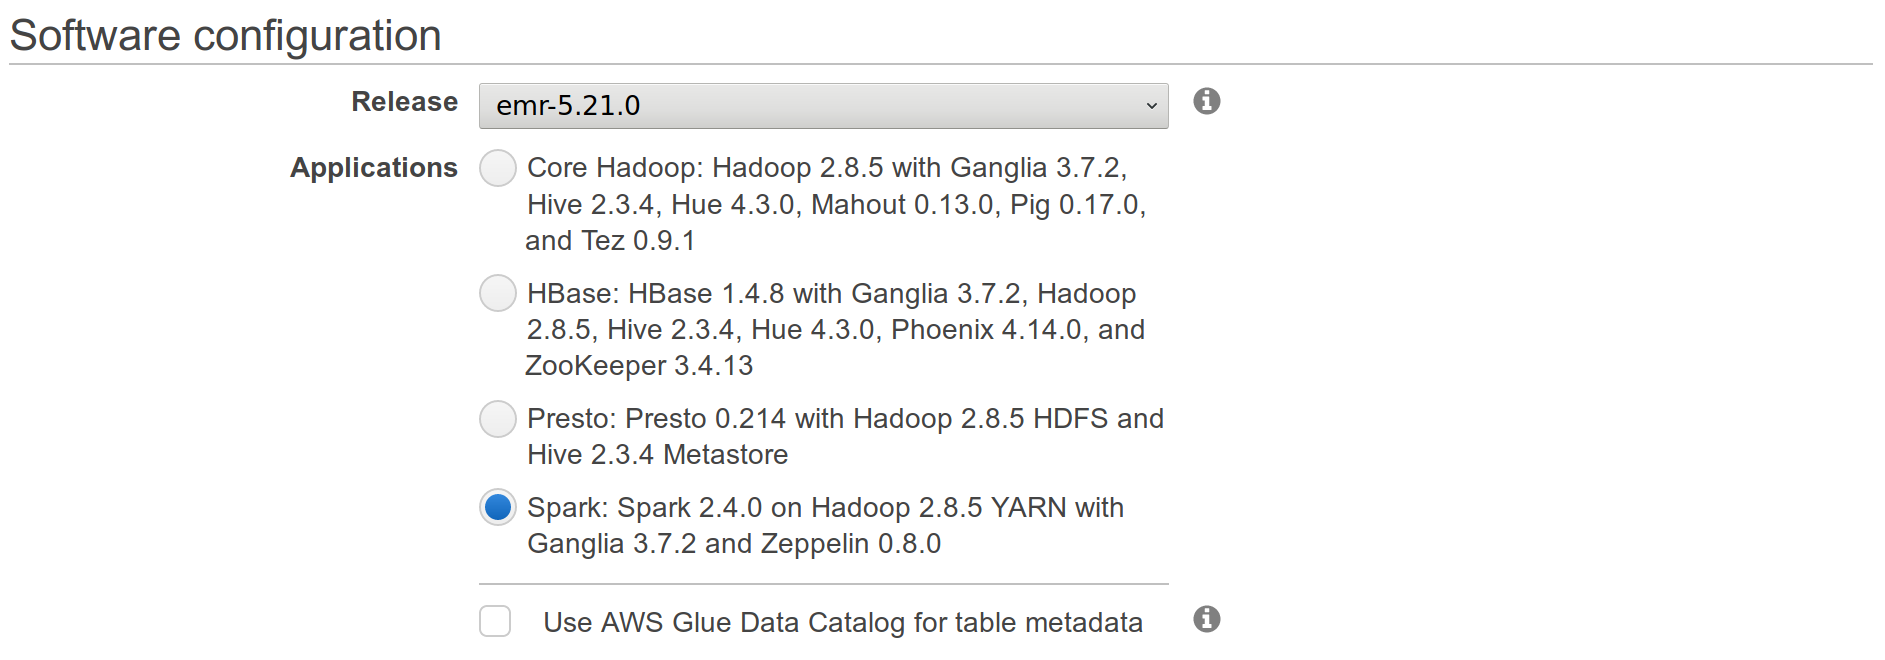
\includegraphics[width=0.8\linewidth]{./figs/aws-emr-spark.png}
  \caption{Make sure to ask AWS to load your cluster with Spark!}
  \label{fig:aws-emr-spark}
\end{figure}


\section{Connect to Master Node}

We're going to use a terminal to ``ssh'' into your spark master.  If you are 
using Mac or Linux you can use your native terminal application.  If you are
using Windows, you can get to a terminal using Jupyter on ORION.

\subsection{Identifying Master Node's Domain}

On the ``Summary'' tab after creating the cluster, locate the section that 
lists your master node's Public DNS, shown in Figure \ref{fig:aws-master-dns}.

\begin{figure}[htpb]
  \centering
  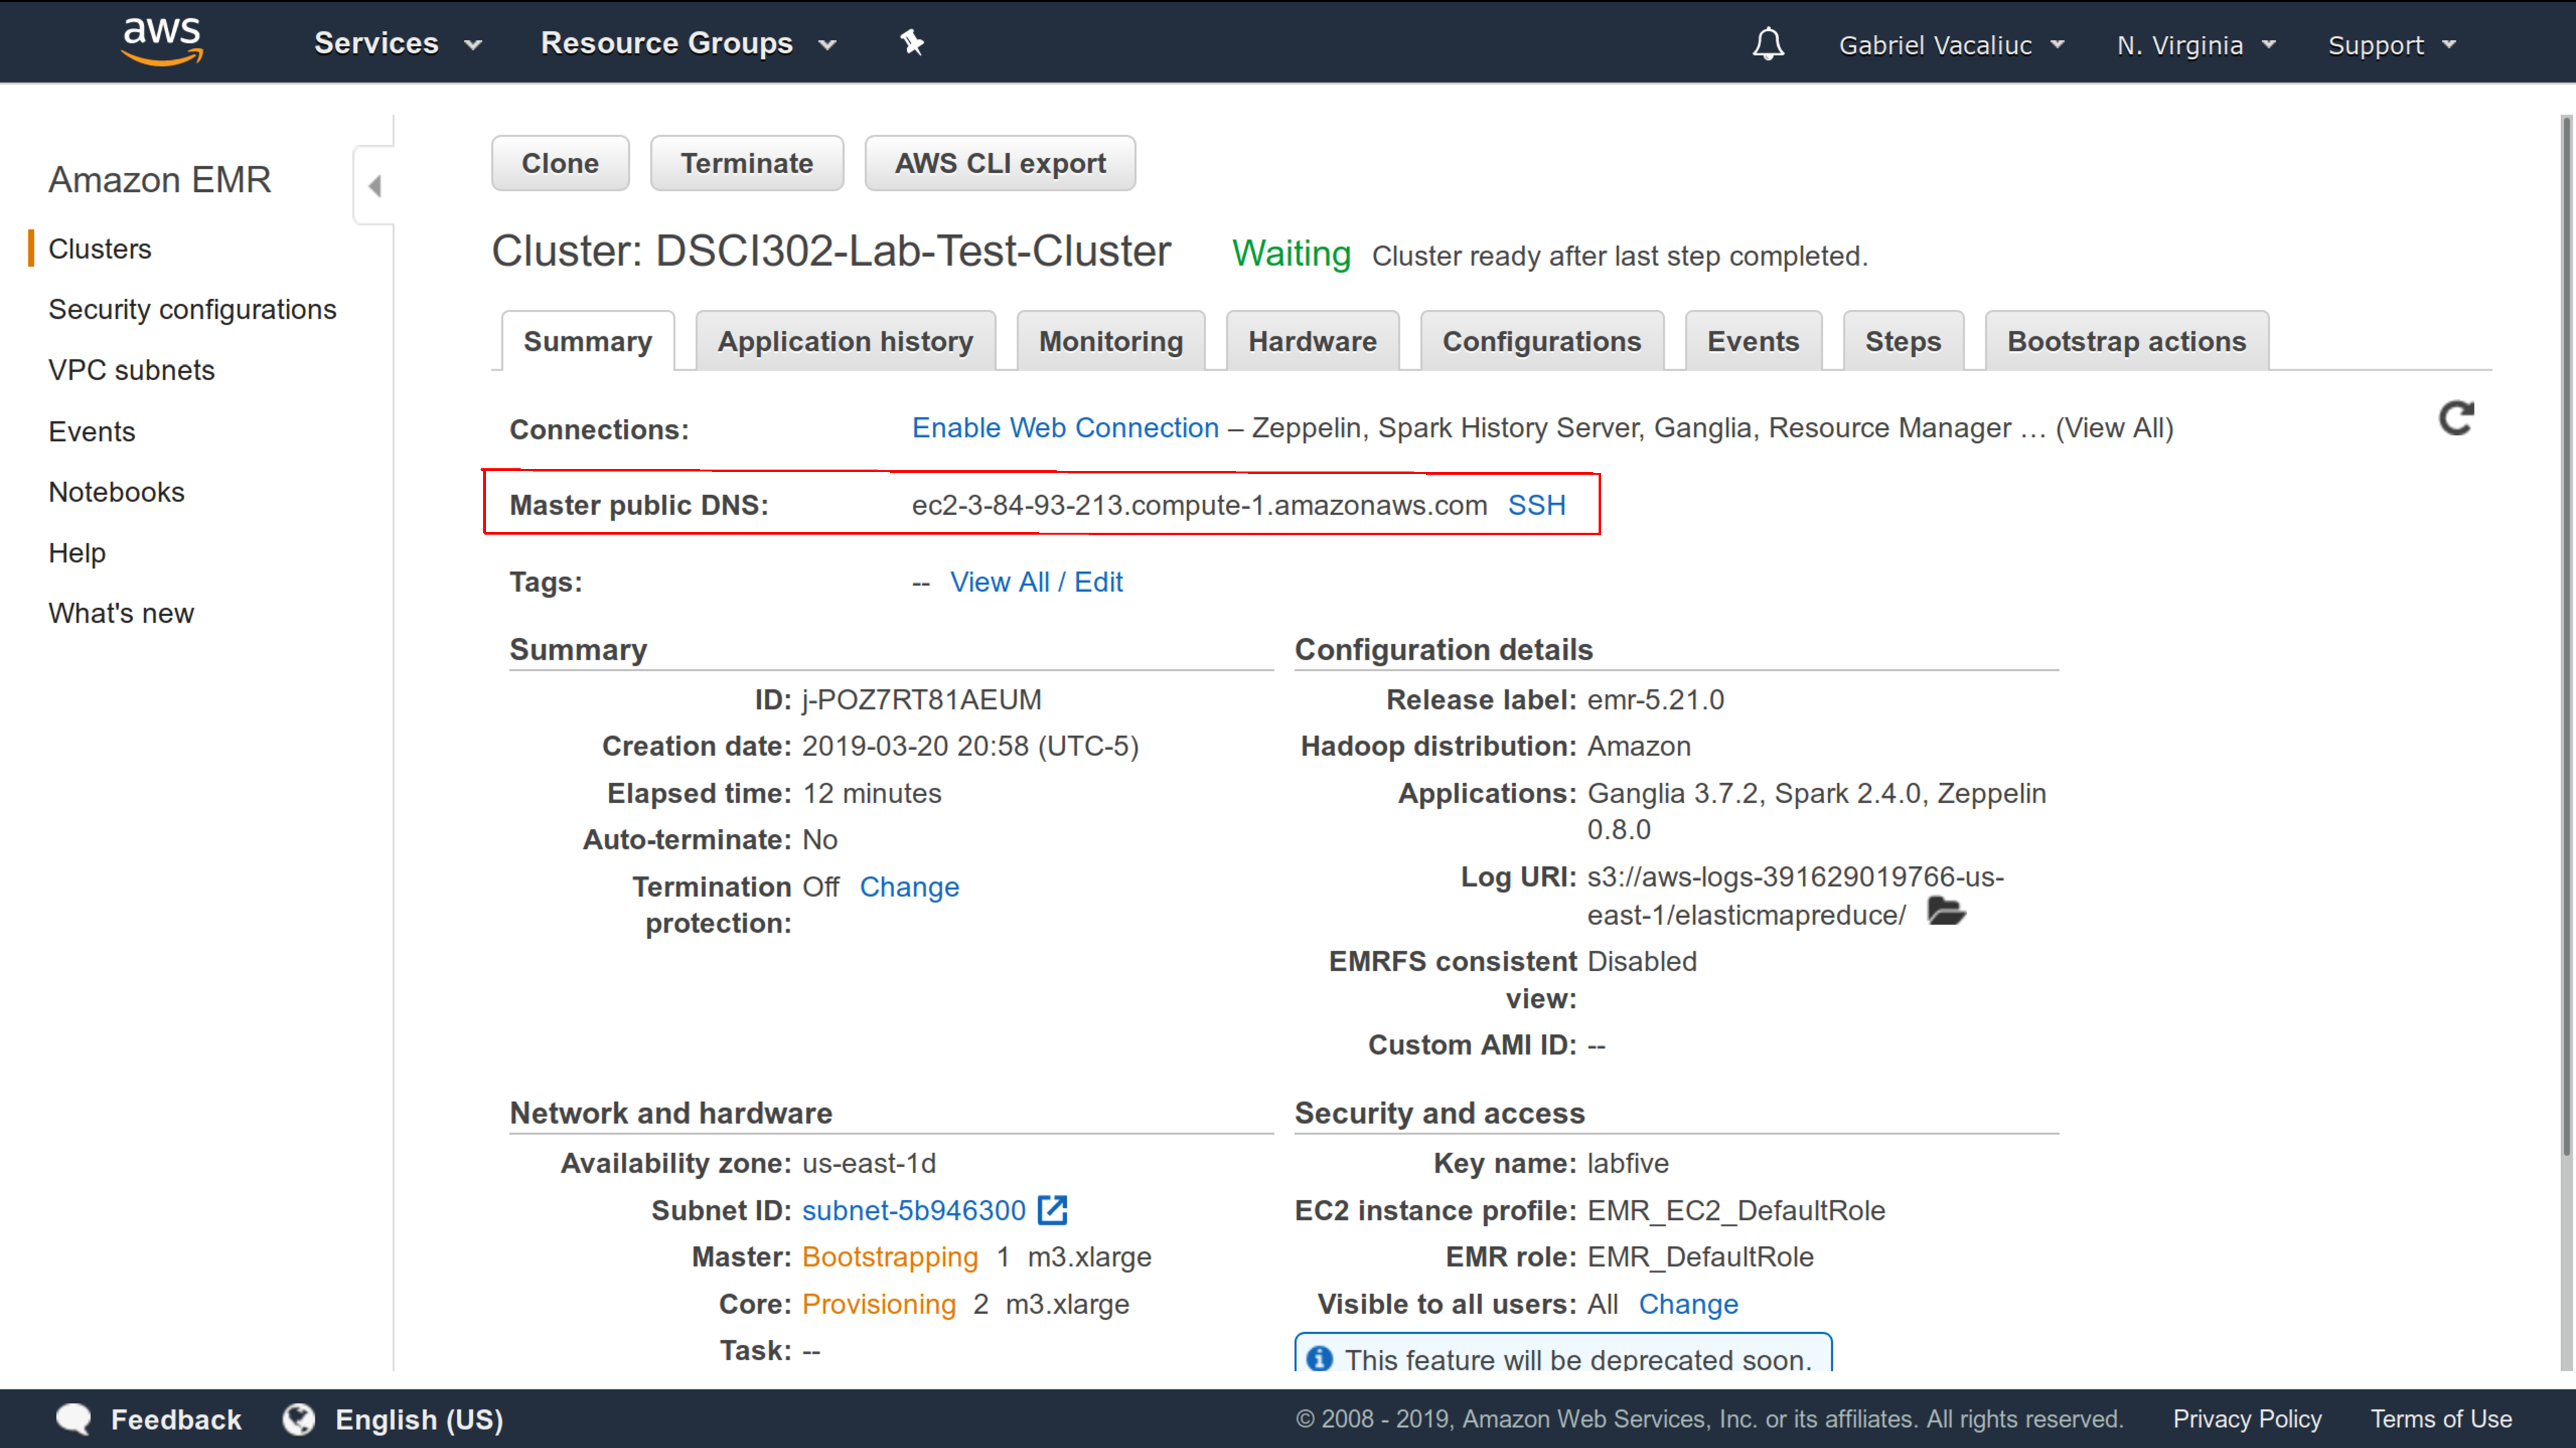
\includegraphics[width=0.8\linewidth]{./figs/aws-emr-dns.pdf}
  \caption{Where to find your master node's Public DNS.}
  \label{fig:aws-master-dns}
\end{figure}

\subsection{Creating a terminal on Jupyter}

To create a terminal on Jupyter, simply launch a server from the
\texttt{gvacaliuc/db-notebook} image, and select New $\rightarrow$ Terminal,
shown in Figure
\ref{fig:jupyter-new-terminal}

\begin{figure}[htpb]
  \centering
  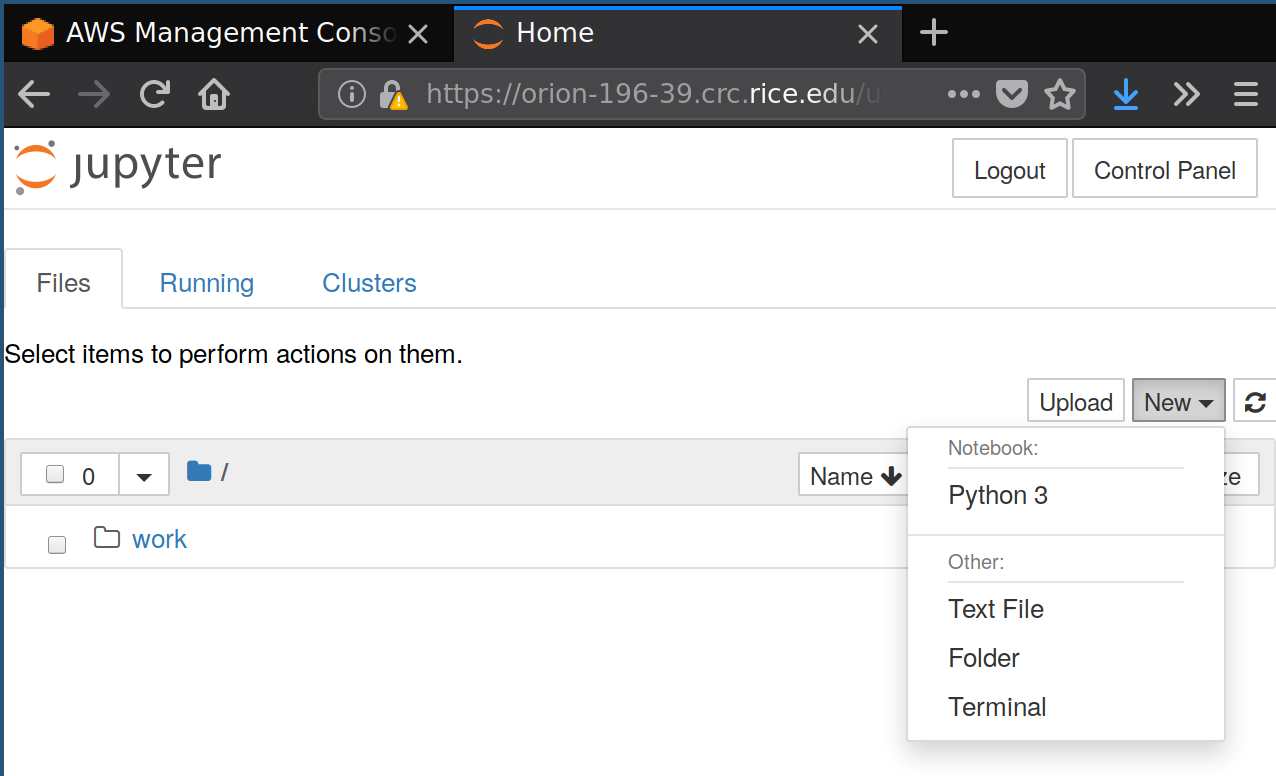
\includegraphics[width=0.4\linewidth]{./figs/jupyter-new-terminal.png}
  \caption{How to create a new terminal from the Jupyter file tree.}
  \label{fig:jupyter-new-terminal}
\end{figure}

\subsection{Connecting from your terminal}

The following assumes that your .pem file is called MyFirstKeyPair.pem;
\textbf{replace this name with the actual name and location of your file},
assuming that you called your key pair something else. Type:

\begin{verbatim}
  chmod 600 MyFirstKeyPair.pem
\end{verbatim}

Now, you can connect to your master machine.  For convenience later, you can
set some environment variables, then connect using ssh and your private key:
\begin{verbatim}
PUBLIC_DNS=ec2-3-84-93-213.compute-1.amazonaws.com # REPLACE THIS WITH YOUR DNS

PRIV_KEY=/path/to/MyFirstKeyPair.pem # REPLACE THIS WITH YOUR PATH

ssh -i $PRIV_KEY hadoop@$PUBLIC_DNS
\end{verbatim}

This will give you a Linux prompt on your cluster's master. You can exit the
remote machine by typing \texttt{exit} at the prompt.

\section{Run Spark jobs}

It is time to run a Spark job!  There are two ways to do this. We will use both.


\begin{enumerate}
\item Submit a Spark job
\begin{enumerate}
  \item Download the file ``topWords.py'' from Canvas and save it in your work
    directory.  If you're working on the ORION terminals, please upload this
    file there.
  \item Open a new terminal in the directory you've been working from (either on ORION or your local machine)
  \item Copy the ``topWords.py'' file to the remote server:
\begin{footnotesize}
\begin{verbatim}
scp -i MyFirstKeyPair.pem /path/to/topWords.py hadoop@$PUBLIC_DNS:~/topWords.py
\end{verbatim}
\end{footnotesize}
  \item Now run the job! From the command line on the remote machine (follow
    instructions above to connect if you have since exited), simply type:
\begin{verbatim}
spark-submit topWords.py
\end{verbatim}
  This will launch the Spark job. A bunch of information will scroll by. After a
  few seconds, the computation is done.
\item Check out your results. Type:
  \begin{verbatim}
    hadoop fs -ls output
  \end{verbatim}
And you will see something like:
\begin{verbatim}
Found 5 items
-rw-r--r--   1 hadoop hadoop          0 2018-10-01 02:39 output/_SUCCESS
-rw-r--r--   1 hadoop hadoop      90587 2018-10-01 02:39 output/part-00000
-rw-r--r--   1 hadoop hadoop      95356 2018-10-01 02:39 output/part-00001
-rw-r--r--   1 hadoop hadoop     101621 2018-10-01 02:39 output/part-00002
-rw-r--r--   1 hadoop hadoop      92673 2018-10-01 02:39 output/part-00003
\end{verbatim}
\item Copy the results from HDFS to the master node. Type:

 \begin{verbatim}
hadoop fs -get output
\end{verbatim}

\item You can have a look at some of the results by typing:
 \begin{verbatim}
more output/part-00001
\end{verbatim}

\item To download the file, use scp again to retrieve the desired files. Note the ``.'' at the end. This copies the specified file to ``here'', your current location.

\begin{footnotesize}
\begin{verbatim}
scp -i MyFirstKeyPair.pem  hadoop@$PUBLIC_DNS:output/part-00000 .
\end{verbatim}
\end{footnotesize}

\item Show one of the graders this file to get checked off.

\end{enumerate}
\item Work with Spark interactively

\begin{enumerate}
  \item Copy the \texttt{countWords.py} file up to the remote machine.  (follow
    the instructions above we used for uploading \texttt{topWords.py}).  Note that this
    should be done from a ``local" terminal.
  \item At a terminal on the remote machine (follow instructions above if you
    have since exited), type \texttt{pyspark}. This starts spark and makes the
    spark context available in your environment as: \texttt{sc}.
  \item Now, import the \texttt{countWords} method from \texttt{countWords.py}:
  
    \texttt{>>> from countWords import countWords}

  \item Then, run the following command:
   {\footnotesize \texttt{countWords(sc, "s3://[DataLocation]/Holmes.txt")}}
    \end{enumerate}
\end{enumerate}


\section{SHUT DOWN YOUR CLUSTER}

{\bf Important: never leave your cluster up when you are not using it. You are being charged!}
\begin{enumerate}
\item From the web page for your cluster, click ``Terminate''.

\item If ``Termination Protection'' is on, you will have to turn it off before you kill your machines.
\item Note: I've had mixed results actually killing machines in this way. After you kill them, make sure that they are dead. Click the cube, click ``EC2'' and click ``Running Instances''. There should not be any. If they are still there, click on ``Running Instances''. Then click the checkbox next to each of your machines, and under ``Actions''-``Instance State'' choose ``terminate''. Only log out after you have verified from the EC2 page that you have no running instances.
\end{enumerate}


\section{FAQ}

\begin{enumerate}
  \item I'm confused.  What terminal should I be running these commands on?

    Generally, we'll be working on the remote machine on AWS, but to open a
    terminal on the remote machine (\texttt{ssh}) and / or copy files to it
    (\texttt{scp}), we'll need to use a terminal on your local computer or
    ORION.  So, basically anytime you're running \texttt{ssh} or \texttt{scp}
    you should be doing this on a ``local" terminal, and AFTER you open a remote
    terminal using \texttt{ssh} to the AWS machine, you should be executing
    commands (\texttt{spark-submit}, \texttt{pyspark}, \texttt{hadoop fs ...})
    on the remote terminal.
\end{enumerate}

\end{document}
